\subsection{Attitude Controller}
The attitude controller for the quadcopter has been designed using a state space representation of the system. This helps handling the coupled angular response of the quadcopter. The chosen states for the system are the three angular positions and the three angular velocities. The input vector of the attitude system consists of the four motor rotational speeds and the output vector consists of the three angles, roll, pitch and yaw. Below, the state, input and the output vectors are presented.
%
\begin{flalign}
	\vec{x}(t) = 
	\begin{bmatrix}
		\phi & \theta & \psi & \dot{\phi} &	\dot{\theta} & \dot{\psi} \\
	\end{bmatrix}	\nonumber
	^T
	\label{xVector}
\end{flalign}  
\begin{flalign}
	\vec{y}(t) = 
	\begin{bmatrix}
		\phi &	\theta & \psi \\
	\end{bmatrix}	\nonumber
	^T
	\label{yVector}
\end{flalign}
\begin{flalign}
	\vec{u}(t)= 
	\begin{bmatrix}
		\omega_1 & \omega_2 &	\omega_3 &	\omega_4 \\
	\end{bmatrix}\nonumber	
	^T
	\label{uVector}+
\end{flalign}
%
The above is then used in construction of the state space matrix representation as displayed in \autoref{xDotSS} and \ref{ySS}.
\begin{flalign}
	\vec{\dot{x}}(t)&=\vec{A} \cdot \vec{x}(t) + \vec{B} \cdot \vec{u}(t)
	\label{xDotSS} 
\end{flalign}
\begin{flalign}
	\vec{y}(t)&=\vec{C} \cdot \vec{x}(t) + \vec{D} \cdot \vec{u}(t)\label{ySS} 
\end{flalign}

Where $\vec{A}$ is the system matrix, $\vec{B}$ is the input matrix, $\vec{C}$ is the output matrix and $\vec{D}$ is the feedback matrix.

The values for the $\vec{A}$, $\vec{B}$, $\vec{C}$ and $\vec{D}$ matrices are obtained from the linearized attitude equations, yielding the matrices shown below. As $\vec{D}$ is a zero matrix, only $\vec{A}$, $\vec{B}$ and $\vec{C}$ are shown. 
\footnotesize
\begin{flalign}   \label{Amatrix}
	\vec{A}=
	\begin{bmatrix}
		\ 0 & 0 & 0 & 1 & 0 & 0     \ \ \ \\ 
		\ 0 & 0 & 0 & 0 & 1 & 0     \ \ \ \\ 
		\ 0 & 0 & 0 & 0 & 0 & 1     \ \ \ \\
		\ 0 & 0 & 0 & 0 & 0 & 0     \ \ \ \\ 
		\ 0 & 0 & 0 & 0 & 0 & 0     \ \ \ \\ 
		\ 0 & 0 & 0 & 0 & 0 & 0     \ \ \  		
	\end{bmatrix}\nonumber
\end{flalign} \label{Bmatrix}
\begin{flalign}
    \vec{B} =
	\begin{bmatrix}
		\ 0 & 0 & 0 & 0      \ \ \ \\ 
		\ 0 & 0 & 0 & 0      \ \ \ \\ 
		\ 0 & 0 & 0 & 0      \ \ \ \\
		\ 0 & \si{-\frac{2 \cdot k_{th} \cdot L \cdot \overline{\omega}_2}{J_x}} & 0 & \si{\frac{2 \cdot k_{th} \cdot L \cdot \overline{\omega}_4}{J_x}}      \ \ \ \\ 
		\ \si{\frac{2 \cdot k_{th} \cdot L \cdot \overline{\omega}_1}{J_y}} & 0 & \si{-\frac{2 \cdot k_{th} \cdot L \cdot \overline{\omega}_3}{J_y}} & 0      \ \ \ \\ 
		\ \frac{2 \cdot k_d \cdot {\overline{\omega}_1}}{J_z} & - \frac{2 \cdot k_d \cdot {\overline{\omega}_2}}{J_z} & \frac{2 \cdot k_d \cdot {\overline{\omega}_3}}{J_z} & - \frac{2 \cdot k_d \cdot {\overline{\omega}_4}}{J_z}      \ \ \ 		
	\end{bmatrix}\nonumber
\end{flalign}
\begin{flalign} \label{Cmatrix}
	\vec{C} =	 
	\begin{bmatrix}
		\ 1 & 0 & 0 & 0 & 0 & 0     \ \ \ \\ 
		\ 0 & 1 & 0 & 0 & 0 & 0     \ \ \ \\ 
		\ 0 & 0 & 1 & 0 & 0 & 0     \ \ \ 		
	\end{bmatrix}\nonumber
\end{flalign}
\normalsize

This system can also be proven to be both controllable and observable, which are necessary conditions to be able to design a observer-based control.

For the quadcopter to hover, it is desired to keep the attitude in equilibrium; this is achieved using a state feedback. To be able to change and track a reference an integral controller is designed combined with the other one. It is also desirable to use an observer in order to estimate the angular velocities that are part of the state of the system. This is done using a reduced-order observer. These two designs can be done independently due to the separation principle. \cite{ssReference}

\autoref{AttitudeControlDiagram} shows how this designs are related.

\begin{figure}[H]
    \centering
    \includegraphics[scale=0.3]{figures/AttitudeControlDiagram}
    \caption{ Control structure for the system, including the state feedback, the integral control and the reduced order observer.}
    \label{AttitudeControlDiagram}
\end{figure}

%--------------------- StateFeedback with Integral Control ----------------------------
The control design is shown in \autoref{fig:DetailedControllerColorDiagram}.
\begin{figure}[H]
    \includegraphics[scale=.35]{figures/DetailedControllerColorDiagram}
    \centering
    \captionof{figure}{Detail of the left diagram, that includes all the variables used in the design of the controller.}
    \label{fig:DetailedControllerColorDiagram}
\end{figure}

It can be seen that there are three new states that are added to the system, $\vec{x}_{Int}(t)$ and lead to the extended system shown in \autoref{xdotSSExtended} and \ref{ySSExtended}.
%
\begin{flalign} 
\dot{\vec{x}}_e(t) &= \vec{A}_e \  \vec{x}_e(t) + \vec{B}_e \  \vec{u}(t) + 
\begin{bmatrix}
\ \vec{0}     \ \ \ \\ 
\ \vec{-I}     \ \ \  		
\end{bmatrix}
\vec{r}(t) 
\label{xdotSSExtended}\\ 
\vec{y}(t) &= \vec{C}_e \  \vec{x}_e 
\label{ySSExtended}
\end{flalign} 
%
being\\
\scriptsize
\begin{minipage}{0.28\linewidth}
    \begin{flalign}
    \dot{\vec{x}}_e(t)= 
    \begin{bmatrix}
    \ \dot{\vec{x}}(t)      \ \  \\ 
    \ \dot{\vec{x}}_{Int}(t)      \ \   		
    \end{bmatrix} \nonumber
    \end{flalign}
\end{minipage}\hfill
\begin{minipage}{0.2\linewidth}
    \begin{flalign}
    \vec{A}_e=
    \begin{bmatrix}
    \ \vec{A}  & \vec{0}    \ \  \\ 
    \ \vec{C}  & \vec{0}    \ \   		
    \end{bmatrix} \nonumber
    \end{flalign}
\end{minipage}   \hfill 
\begin{minipage}{0.2\linewidth}
    \begin{flalign}
    \vec{B}_e=
    \begin{bmatrix}
    \ \vec{B}    \ \  \\ 
    \ \vec{0}     \ \   		
    \end{bmatrix} \nonumber
    \end{flalign}
\end{minipage}\hfill
\begin{minipage}{0.2\linewidth}
    \begin{flalign}
    \vec{C}_e=
    \begin{bmatrix}
    \ \vec{C}  & \vec{0}  \ \   		
    \end{bmatrix} \nonumber
    \end{flalign}
\end{minipage}
\normalsize
\\

With this approach, the control law given by \autoref{eq:ssControllerAction}.
%
\begin{flalign} 
    \vec{u}(t) &=\vec{F} \  \vec{x}(t) + \ \vec{F}_{Int} \  \vec{x}_{Int}(t)
    \label{eq:ssControllerAction}
\end{flalign}
%
The resulting feedback law can be design as a conventional state feedback, where the goal is to choose an appropriate $F_e=[F \ F_{Int}]$ matrix such that the eigenvalues of $A_e+B_eF_e$ are the new poles that the system needs to have in order to achieve the desired dynamics.

Once $F_e$ is obtained, it can be split into $F$ and $F_{Int}$ by taking the first 6 columns for the state feedback and the last 3 for the integral control. In this way, the controller can be implemented as shown in \autoref{fig:DetailedControllerColorDiagram}.

%--------------------- Reduced-Order Observer ----------------------------


In general an observer is utilized in a control system if either one of two specific cases occurs. If certain states in the system are not measured, an observer can estimate the unmeasured states by means of the system output and input. However, it is also possible to use an observer if the measured data gathered from the sensors is affected by noise. The observer can thereby use both the noisy measured states and the estimated states creating a filtered version. This case will however not be utilized in the prototype.

With this approach, the first three states, $x_1$ with be equal to the outputs, $y$, whereas the other three states will be estimated, $\hat{x}_2$.

The matrices that define the original system can be split into submatrices, that will be used in the design of the observer, as follows:\\
%
\begin{minipage}{0.45\linewidth}
    \begin{flalign}
    \vec{A}=
    \begin{bmatrix}
    \ \vec{A11}_{3 \times 3}  & \vec{A12}_{3 \times 3}    \ \ \ \\ 
    \ \vec{A21}_{3 \times 3}  & \vec{A22}_{3 \times 3}    \ \ \  		
    \end{bmatrix} \nonumber
    \end{flalign}
\end{minipage}   \hfill 
\begin{minipage}{0.45\linewidth}
    \begin{flalign}
    \vec{B}=
    \begin{bmatrix}
    \ \vec{B1}_{3 \times 4}    \ \ \ \\ 
    \ \vec{B2}_{3 \times 4}     \ \ \  		
    \end{bmatrix} \nonumber
    \end{flalign}
\end{minipage}\hfill
\\

As described in ?? the system is observable, making it possible to find an observer gain, $L_{obs}$, which makes \autoref{eq:observerStable} stable \cite{ssReference}.
%
\begin{flalign}
    \vec{A_{22}} + \vec{L_{obs}}\vec{A_{A12}} \label{eq:observerStable}
\end{flalign}

With this observer gain, the observer in \autoref{eq:observerStable} ensures an estimate $\hat{x}_2$ which converges to $x_2$ at a rate given by the eigenvalues of \autoref{eq:eqobservertheorem}.
\small
\begin{flalign}
    \vec{\hat{\dot{x}}_2} &= \vec{A_{21}}\vec{y} + \vec{A_{22}}\vec{\hat{x}_2} + \vec{B_2u} + \vec{L_{obs}}\vec{(A_{12}\hat{x}_2} - \vec{A_{21}x_2}) \label{eq:eqobservertheorem}
\end{flalign}
\normalsize \\
This estimation of $\hat{x}_2$ can also be seen\autoref{fig:observerDiagram}.
\begin{figure}[H]
    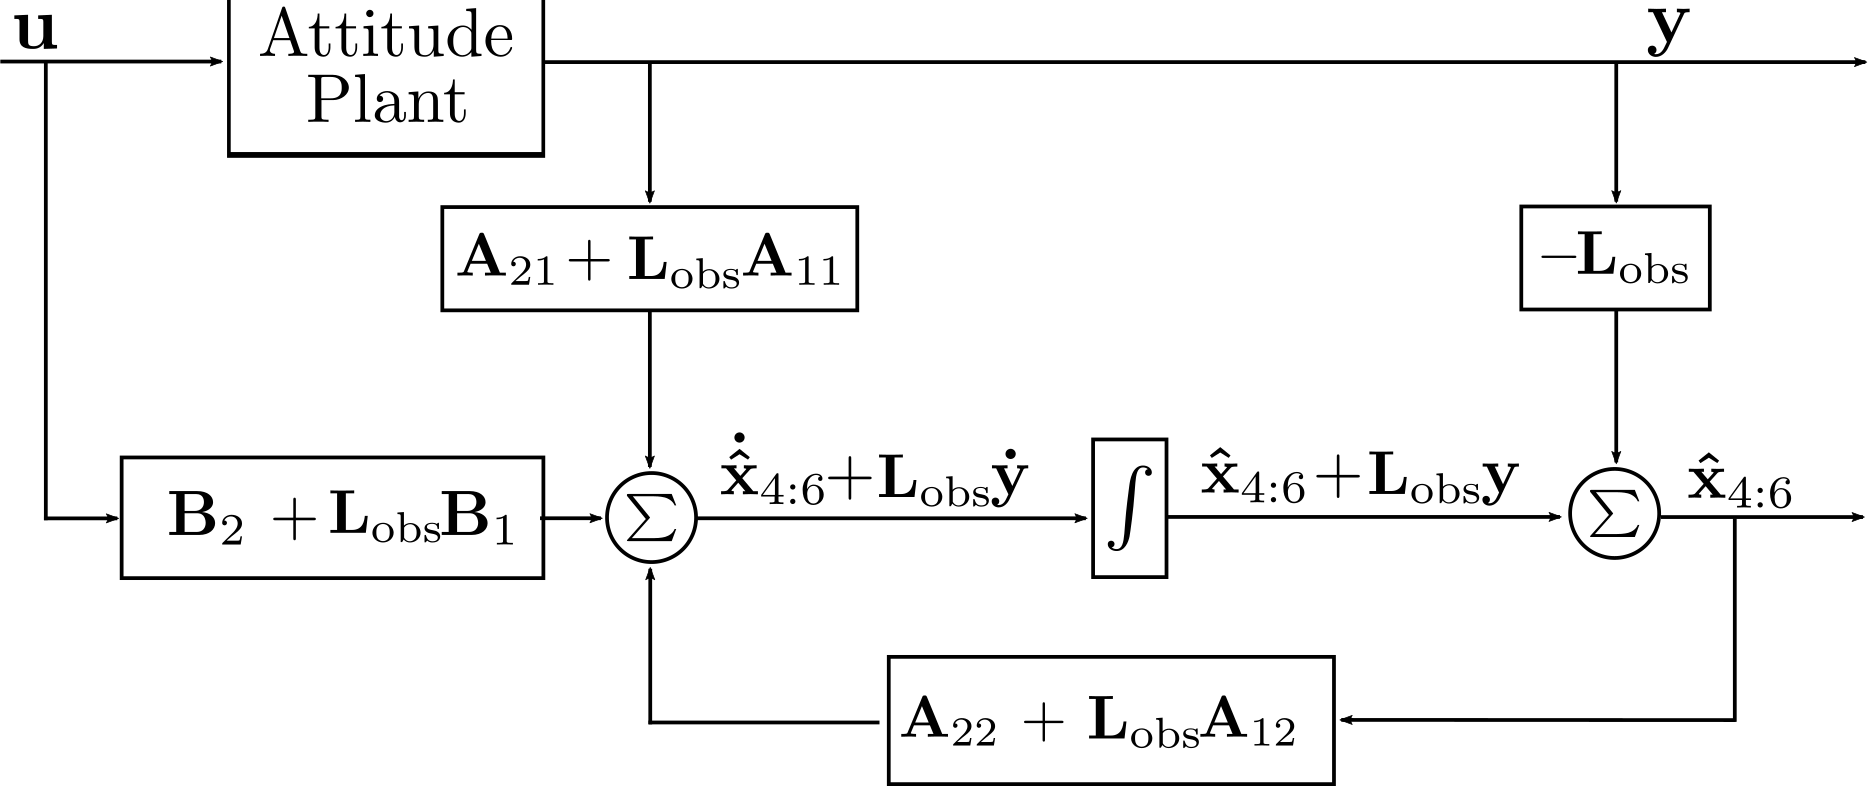
\includegraphics[scale=.2]{figures/observerDiagram}
    \centering
    \captionsetup{justification=centering}
    \captionof{figure}{This diagram should be made so it looks a bit more similar to the previous on. But only the part with the observer.}
    \label{fig:observerDiagram}
\end{figure}











